






% =========----------	[ Space left here for distraction free mode] ----------==========%










\section{Literature Review} \label{lit}

	This section will provide an overview of the necessary literature upon which this project is based. \\

	\subsection{Ambisonics}

		Originally conceived by Gerzon \cite{gerzon1973} in the 1970's, Ambisonics is a technique that exploits the decomposition of sound fields into spherical harmonics for spatial audio reproduction. At its most basic form, First Order Ambisonics (FOA) can be used to reproduce a 3-dimensional sound field using just four spherical harmonic components. This can then be extended to Higher Order Ambisonics (HOA) which includes spherical harmonic components beyond the first order which increases sound field reproduction accuracy \cite{Bertet2007}. A major benefit of the Ambisonics framework is that the number of channels required is determined only by the Ambisonic order as opposed to the number of sound sources to be encoded. Further still, when using loudspeakers for the sound field reproduction, the number of loudspeakers required is variable depending on the Ambisonic order. An Ambisonic signal can be decoded over a variety of different loudspeaker configurations providing that the number of loudspeakers is equal or greater than the number of spherical harmonics, $m =(n+1)^2$ where $n$ is the Ambisonic order. Ambisonic can be decoded for binaural playback over headphones by using \textit{virtual loudspeakers}, where a HRTF data set is used in place of real loudspeakers. Combining this with a dynamically rotating sound field, accurate real world listening can be reproduced over headphone \cite{Mckeag1996} \cite{Noisternig2003}. \\

		Recording spatial audio to use for an Ambisonics framework can be done using multiple different recording techniques. These will be covered in the following sections.


	\subsection{Ambisonic Microphones}

		\subsubsection{FOA Microphones}

			There are two commercially available FOA microphones available on the market that are used in this study, the \textbf{Soundfield ST450 MKII} and the \textbf{Sennheiser AMBEO VR Microphone}. Both microphones utilise a coincident tetrahedral arrangement of four cardioid microphone capsules to capture the sound pressure on the surface of a sphere. The four channel output from the microphones containing the raw audio captured by the four microphone capsules is known as A-Format and is converted into a B-Format signal by summing and subtracting the audio signals in various ways to produce a omni directional channel (W) and three figure of 8 channels (X,Y,Z) \cite{Power}.

		\subsubsection{HOA Microphones}

			Following the same principle as FOA microphones, HOA microphones capture the sound pressure on the surface of a sphere however a greater number of microphone capsules are used and more complicated algorithms for converting from the raw recorded signal to an Ambisonic signal are required. The HOA microphone used in this study is the Eigenmike consisting of thirty-two omni-directional electret capsules in a pentakis-dodecahedron configuration enabling the Eigenmike to record up to 4\su{th} order Ambisonics \cite{Bates} increasing the spatial resolution beyond that capable of the FOA microphones. Studies have previously shown the Eigenmikes adequate performance regarding directionality however has been rated low in terms of quality \cite{Bates}. This is due to the increased number of microphone capsules creating an unattributable noise floor.


	\subsection{Multichannel Microphones Arrays} \label{lit:microphones}

		Given the vast number of different types of microphones and polar patterns, there are an infinite number of possible microphone array configurations available. The following sections review a selection of multichannel microphone arrays (MMAs) that have been previously purposefully designed for spatial audio capture that were utilised in this study.


		\subsubsection{Equal-Segment-Microphone-Array (ESMA)}
			\begin{figure}[h!]
			\begin{center}
				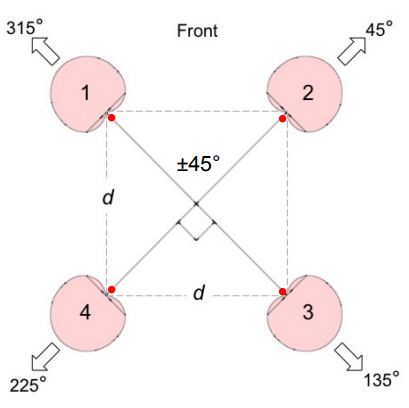
\includegraphics[width = 0.4\linewidth]{images/mic/esma.png}
				\caption{Equal-segment-microphone-array proposed by Michael Williams \cite{esma}}
				\label{esmaSchematic}
			\end{center}
			\end{figure}
			The ESMA was designed to capture sound from 360\textdegree{} in the azimuth plane using four cardioid microphones positioned in a square arrangement, with a distance of 25cm between each capsule. The angles between each microphone should be 90\textdegree{}, creating a stereophonic recording angle (SRA) of $ \pm45 $\textdegree{} \cite{williamsMMAD}, \cite{williams91}. Dr Hyunkook Lee of Huddersfield University found that by changing the distance between each capsule to 50cm, the localisation accuracy of sound sources within a VR environment was improved \cite{esma}. Lee also proposed that an additional four upward-facing cardioid microphones could be added to the array to capture the diffuse sound within the recording environment. The four upward-facing microphones should also have a distance of 50cm between them and are represented by the red dots in Fig. \ref{esmaSchematic}. Inter-channel cross talk is minimised due to the use of spacing and cardioid polar patterns.\\

		\subsubsection{ORTF-3D Surround}

			\begin{figure}[h!]
			\begin{center}
				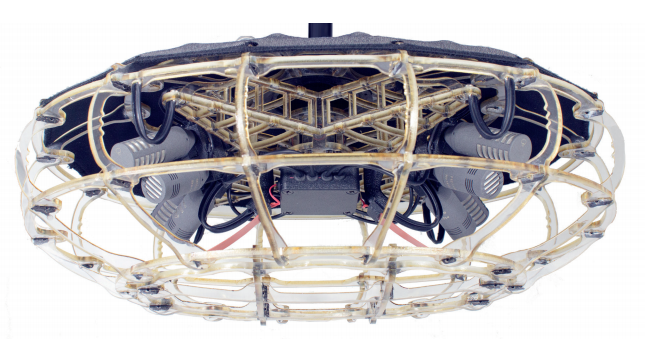
\includegraphics[width = 0.45\linewidth]{images/mic/ortf3D.PNG}
				\caption{ORTF-3D Surround microphone array \cite{ORTF3D2}}
				\label{ORTF3D}
			\end{center}
			\end{figure}

			The ORTF-3D surround is a near-coincident microphone array designed by G\"{u}nther Theile and Helmut Wittek for Schoeps Mikrofone. The bottom plane consists of four supercardioid CCM 41 Schoeps microphones positioned in a 10cm x 20cm rectangle. The capsules are directed to the left front (LF), right front (RF), rear left (LS) and rear right (LR). The angles between the left and right capsules are 80\textdegree{} and 100\textdegree{} between the front and rear capsules. The upper plane consists of four supercardioid CCM 41V Schoeps microphones with the capsules facing upwards (LFh, RFh, LSh and RSh) to create coincident X-Y pairs at 90\textdegree{} between the upper and lower planes \cite{ORTF3D2}. Supercardioid microphones coupled with the spacing between microphones prevent unwanted inter-channel cross talk and comb-filtering effects as well as improved spatial resolution.

		\subsubsection{OCT-9 Surround}
			\label{sec:OCT9}	

			\begin{figure}[h!]
			\begin{center}
				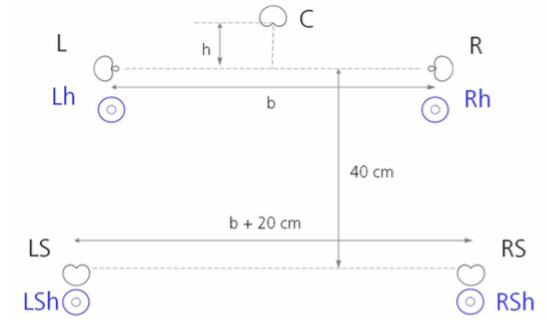
\includegraphics[width = 0.6\linewidth]{images/mic/OCT.png}
				\caption{OCT-9 Surround microphone array \cite{TheileWittek}}
				\label{oct}
			\end{center}
			\end{figure}

			 The OCT-9 Surround microphone array was also designed by G\"{u}nther Theile and Helmut Wittek for the Auro-3D (9.1) loudspeaker arrangement. The front facing section is based on Theile's optimised cardioid triangle surround (OCT-Surround) array, which is used to capture sound for 5.1 multichannel systems \cite{TheileWittek}, \cite{Theile}. This includes four upwards facing supercardioid microphones for diffuse field capture. Each channel should be fed directly to its corresponding loudspeaker in the Auro-3D loudspeaker system.

		\subsubsection{Perspective Control Microphone Array (PCMA)}

			\begin{figure}[h!]
			\begin{center}
				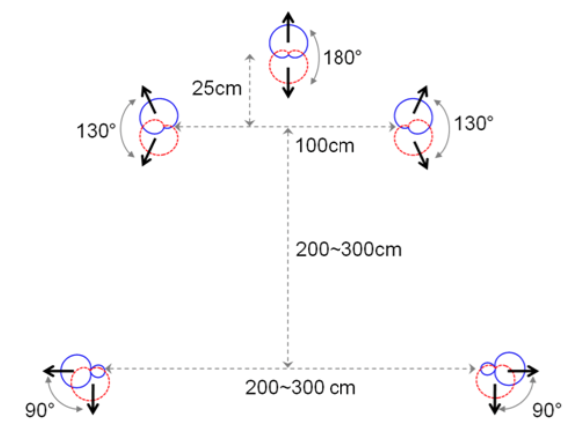
\includegraphics[width = 0.5\linewidth]{images/mic/pcma.png}
				\caption{PCMA arrangement \cite{leePCMA}}
				\label{pcma}
			\end{center}
			\end{figure}
			The PCMA arrangement is similar to OCT-Surround but five widely spaced coincident pairs are used in place of single microphones. Each pair uses cardioid microphones creating virtual microphones through different mixing ratios \cite{leePCMA}. This allows perceived source distance and source width to be changed post-recording \cite{leePCMA}.

		\subsubsection{Hamasaki Cube}

			\begin{figure}[h!]
			\begin{center}
				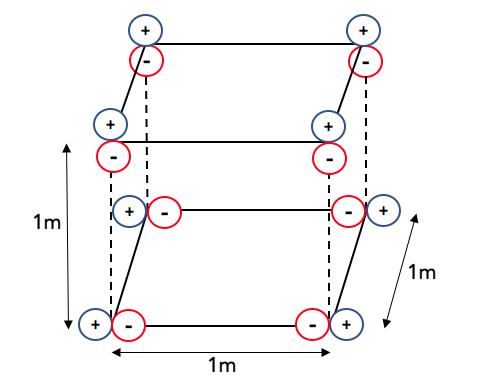
\includegraphics[width = 0.5\linewidth]{images/mic/Hamasaki1.png}
				\caption{Hamasaki Cube Microphone Array}
				\label{ham}
			\end{center}
			\end{figure}

			The Hamasaki Cube microphone array is specifically designed to capture the reverberation and diffuse sound in performance spaces such as concert halls. The array consists of eight bi-directional microphones positioned in a cube arrangement with equal spacing of 1 metre between each microphone. The nulls of each microphone are pointed inwards, which helps to reduce the capture of direct sound. This array is usually used in combination with other direct sound capture arrays to reproduce the full spatial impression of the performance space \cite{TheileWittek}.

		\subsubsection{IRT Cross}

			\begin{figure}[h!]
			\begin{center}
				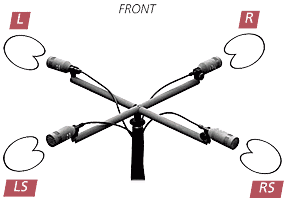
\includegraphics[width = 0.5\linewidth]{images/mic/irt.png}
				\caption{Schoeps IRT Cross microphone array \cite{IRTschoeps}}
				\label{irt}
			\end{center}
			\end{figure}

			The IRT cross array, also known as the 'atmo-cross' is used to capture reflected diffuse sound and direct environmental sounds such as applause and crowd noise\cite{IRTschoeps}. It can be created using four cardioid microphones positioned in a square with 20cm - 25cm spacing between each capsule. The capsules should be facing towards the front left (FL), front right (FR), rear left (LS) and rear right (RS).